% generated by Plantuml 1.2024.4       
\definecolor{plantucolor0000}{RGB}{0,0,0}
\definecolor{plantucolor0001}{RGB}{0,64,115}
\definecolor{plantucolor0002}{RGB}{255,255,255}
\definecolor{plantucolor0003}{RGB}{211,214,222}
\definecolor{plantucolor0004}{RGB}{24,24,24}
\scalebox{0.7171}{
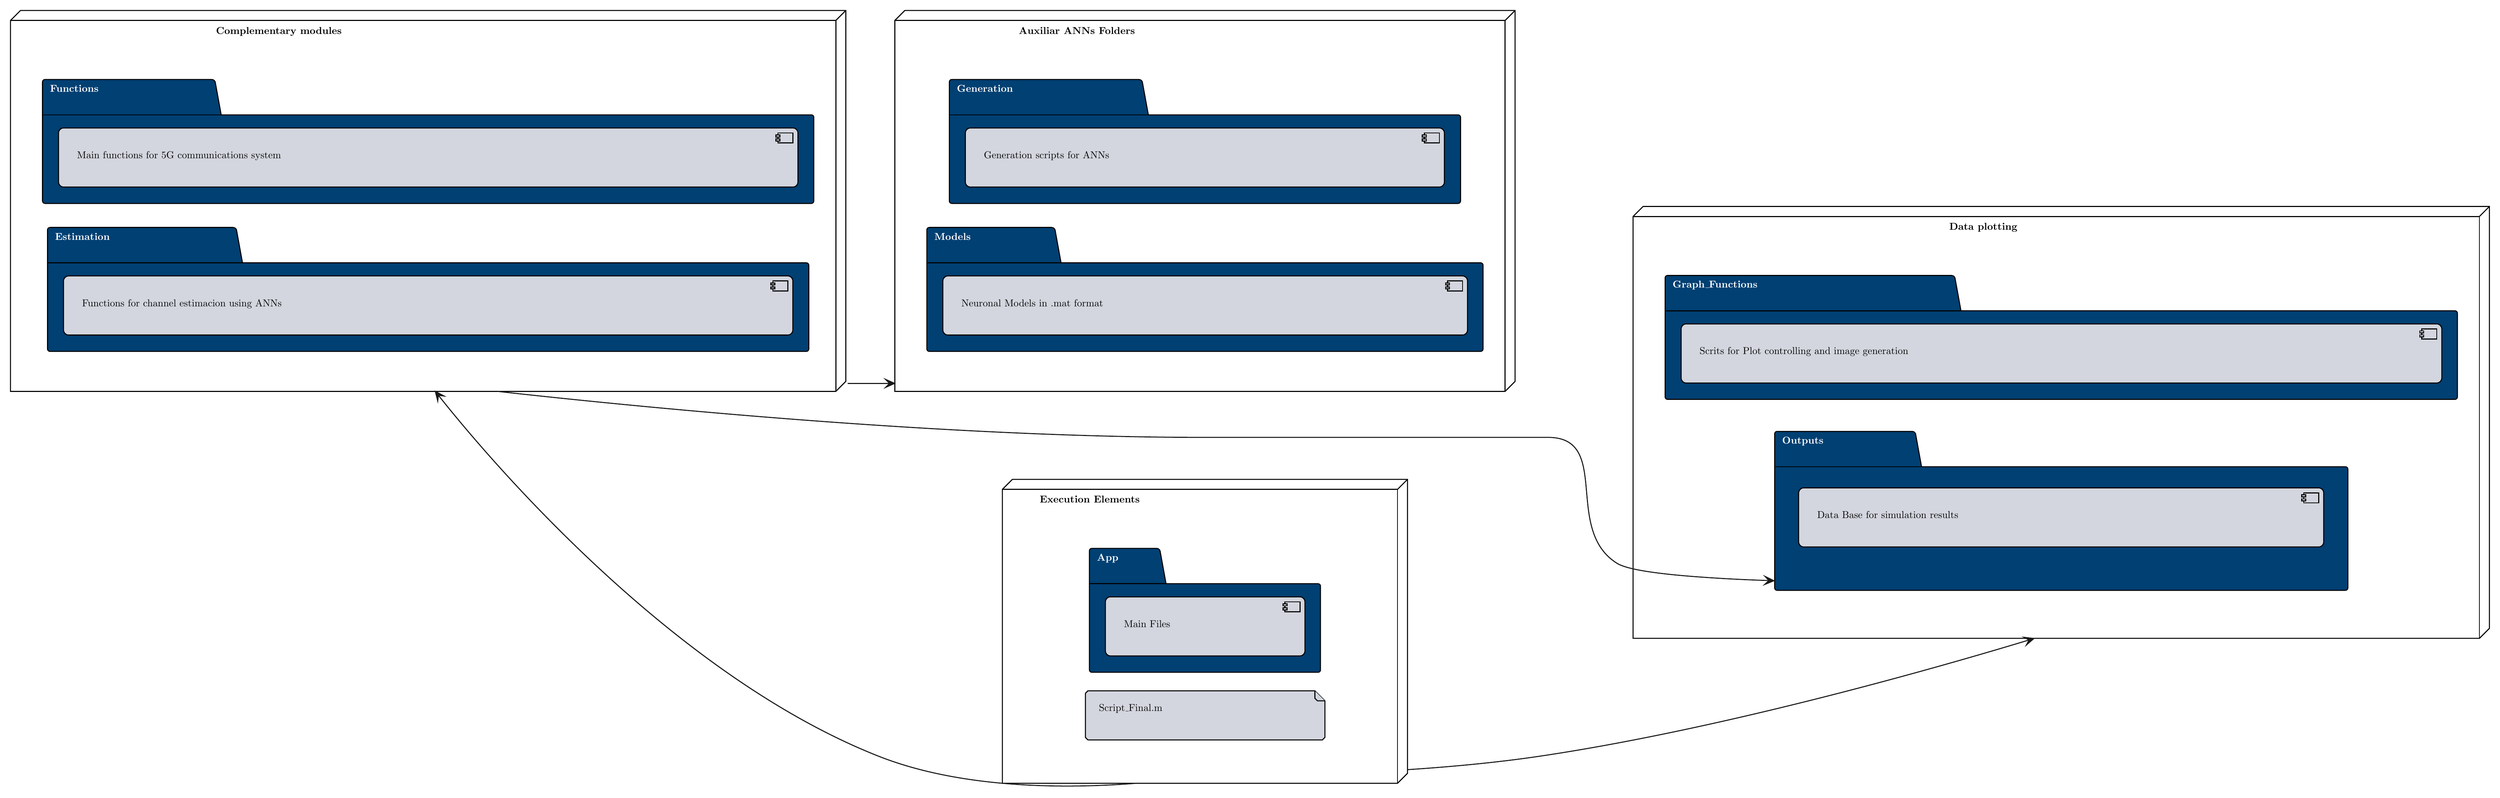
\begin{tikzpicture}[yscale=-1
,pstyle0/.style={color=black,line width=1.0pt}
,pstyle1/.style={color=black,fill=plantucolor0001,line width=1.0pt}
,pstyle2/.style={color=black,fill=plantucolor0003,line width=1.0pt}
,pstyle3/.style={color=plantucolor0004,line width=1.0pt}
,pstyle4/.style={color=plantucolor0004,fill=plantucolor0004,line width=1.0pt}
]
\draw[pstyle0] (1638pt,212pt) -- (1648pt,202pt) -- (2494pt,202pt) -- (2494pt,624pt) -- (2484pt,634pt) -- (1638pt,634pt) -- (1638pt,212pt) -- cycle;
\draw[pstyle0] (2484pt,212pt) -- (2494pt,202pt);
\draw[pstyle0] (1638pt,212pt) -- (2484pt,212pt);
\draw[pstyle0] (2484pt,212pt) -- (2484pt,634pt);
\node at (1950.6362pt,215pt)[below right,color=black]{\textbf{Data plotting}};
\draw[pstyle1] (1672.5pt,271pt) -- (1956.2261pt,271pt) arc(270:360:3.75pt)  -- (1965.7261pt,306.3701pt) -- (2459.5pt,306.3701pt) arc(270:360:2.5pt)  -- (2462pt,392.5pt) arc(0:90:2.5pt)  -- (1672.5pt,395pt) arc(90:180:2.5pt)  -- (1670pt,273.5pt) arc(180:270:2.5pt) ;
\draw[pstyle0] (1670pt,306.3701pt) -- (1965.7261pt,306.3701pt);
\node at (1674pt,273pt)[below right,color=white]{\textbf{Graph\_Functions}};
\draw[pstyle1] (1782pt,427pt) -- (1916.8301pt,427pt) arc(270:360:3.75pt)  -- (1926.3301pt,462.3701pt) -- (2350pt,462.3701pt) arc(270:360:2.5pt)  -- (2352.5pt,583.5pt) arc(0:90:2.5pt)  -- (1782pt,586pt) arc(90:180:2.5pt)  -- (1779.5pt,429.5pt) arc(180:270:2.5pt) ;
\draw[pstyle0] (1779.5pt,462.3701pt) -- (1926.3301pt,462.3701pt);
\node at (1783.5pt,429pt)[below right,color=white]{\textbf{Outputs}};
\draw[pstyle0] (900pt,16pt) -- (910pt,6pt) -- (1520pt,6pt) -- (1520pt,377pt) -- (1510pt,387pt) -- (900pt,387pt) -- (900pt,16pt) -- cycle;
\draw[pstyle0] (1510pt,16pt) -- (1520pt,6pt);
\draw[pstyle0] (900pt,16pt) -- (1510pt,16pt);
\draw[pstyle0] (1510pt,16pt) -- (1510pt,387pt);
\node at (1020.3597pt,19pt)[below right,color=black]{\textbf{Auxiliar ANNs Folders}};
\draw[pstyle1] (957pt,75pt) -- (1143.9032pt,75pt) arc(270:360:3.75pt)  -- (1153.4032pt,110.3701pt) -- (1463pt,110.3701pt) arc(270:360:2.5pt)  -- (1465.5pt,196.5pt) arc(0:90:2.5pt)  -- (957pt,199pt) arc(90:180:2.5pt)  -- (954.5pt,77.5pt) arc(180:270:2.5pt) ;
\draw[pstyle0] (954.5pt,110.3701pt) -- (1153.4032pt,110.3701pt);
\node at (958.5pt,77pt)[below right,color=white]{\textbf{Generation}};
\draw[pstyle1] (934.5pt,223pt) -- (1056.6451pt,223pt) arc(270:360:3.75pt)  -- (1066.1451pt,258.3701pt) -- (1485.5pt,258.3701pt) arc(270:360:2.5pt)  -- (1488pt,344.5pt) arc(0:90:2.5pt)  -- (934.5pt,347pt) arc(90:180:2.5pt)  -- (932pt,225.5pt) arc(180:270:2.5pt) ;
\draw[pstyle0] (932pt,258.3701pt) -- (1066.1451pt,258.3701pt);
\node at (936pt,225pt)[below right,color=white]{\textbf{Models}};
\draw[pstyle0] (16pt,16pt) -- (26pt,6pt) -- (851pt,6pt) -- (851pt,377pt) -- (841pt,387pt) -- (16pt,387pt) -- (16pt,16pt) -- cycle;
\draw[pstyle0] (841pt,16pt) -- (851pt,6pt);
\draw[pstyle0] (16pt,16pt) -- (841pt,16pt);
\draw[pstyle0] (841pt,16pt) -- (841pt,387pt);
\node at (217.9291pt,19pt)[below right,color=black]{\textbf{Complementary modules }};
\draw[pstyle1] (50.5pt,75pt) -- (217.1pt,75pt) arc(270:360:3.75pt)  -- (226.6pt,110.3701pt) -- (816.5pt,110.3701pt) arc(270:360:2.5pt)  -- (819pt,196.5pt) arc(0:90:2.5pt)  -- (50.5pt,199pt) arc(90:180:2.5pt)  -- (48pt,77.5pt) arc(180:270:2.5pt) ;
\draw[pstyle0] (48pt,110.3701pt) -- (226.6pt,110.3701pt);
\node at (52pt,77pt)[below right,color=white]{\textbf{Functions}};
\draw[pstyle1] (55.5pt,223pt) -- (238.3909pt,223pt) arc(270:360:3.75pt)  -- (247.8909pt,258.3701pt) -- (811.5pt,258.3701pt) arc(270:360:2.5pt)  -- (814pt,344.5pt) arc(0:90:2.5pt)  -- (55.5pt,347pt) arc(90:180:2.5pt)  -- (53pt,225.5pt) arc(180:270:2.5pt) ;
\draw[pstyle0] (53pt,258.3701pt) -- (247.8909pt,258.3701pt);
\node at (57pt,225pt)[below right,color=white]{\textbf{Estimation}};
\draw[pstyle0] (1007.5pt,485pt) -- (1017.5pt,475pt) -- (1412.5pt,475pt) -- (1412.5pt,769pt) -- (1402.5pt,779pt) -- (1007.5pt,779pt) -- (1007.5pt,485pt) -- cycle;
\draw[pstyle0] (1402.5pt,485pt) -- (1412.5pt,475pt);
\draw[pstyle0] (1007.5pt,485pt) -- (1402.5pt,485pt);
\draw[pstyle0] (1402.5pt,485pt) -- (1402.5pt,779pt);
\node at (1041.3143pt,488pt)[below right,color=black]{\textbf{Execution Elements}};
\draw[pstyle1] (1097pt,544pt) -- (1161.6pt,544pt) arc(270:360:3.75pt)  -- (1171.1pt,579.3701pt) -- (1323pt,579.3701pt) arc(270:360:2.5pt)  -- (1325.5pt,665.5pt) arc(0:90:2.5pt)  -- (1097pt,668pt) arc(90:180:2.5pt)  -- (1094.5pt,546.5pt) arc(180:270:2.5pt) ;
\draw[pstyle0] (1094.5pt,579.3701pt) -- (1171.1pt,579.3701pt);
\node at (1098.5pt,546pt)[below right,color=white]{\textbf{App}};
\draw[pstyle2] (1686pt,324.5pt) arc (180:270:5pt) -- (1691pt,319.5pt) -- (2441.3567pt,319.5pt) arc (270:360:5pt) -- (2446.3567pt,324.5pt) -- (2446.3567pt,373.6016pt) arc (0:90:5pt) -- (2441.3567pt,378.6016pt) -- (1691pt,378.6016pt) arc (90:180:5pt) -- (1686pt,373.6016pt) -- cycle;
\draw[pstyle2] (2426.3567pt,324.5pt) rectangle (2441.3567pt,334.5pt);
\draw[pstyle2] (2424.3567pt,326.5pt) rectangle (2428.3567pt,328.5pt);
\draw[pstyle2] (2424.3567pt,330.5pt) rectangle (2428.3567pt,332.5pt);
\node at (1701pt,339.5pt)[below right,color=black]{Scrits for Plot controlling and image generation};
\draw[pstyle2] (1803.5pt,488.5pt) arc (180:270:5pt) -- (1808.5pt,483.5pt) -- (2323.3538pt,483.5pt) arc (270:360:5pt) -- (2328.3538pt,488.5pt) -- (2328.3538pt,537.6016pt) arc (0:90:5pt) -- (2323.3538pt,542.6016pt) -- (1808.5pt,542.6016pt) arc (90:180:5pt) -- (1803.5pt,537.6016pt) -- cycle;
\draw[pstyle2] (2308.3538pt,488.5pt) rectangle (2323.3538pt,498.5pt);
\draw[pstyle2] (2306.3538pt,490.5pt) rectangle (2310.3538pt,492.5pt);
\draw[pstyle2] (2306.3538pt,494.5pt) rectangle (2310.3538pt,496.5pt);
\node at (1818.5pt,503.5pt)[below right,color=black]{Data Base for simulation results};
\draw[pstyle2] (970.5pt,128.5pt) arc (180:270:5pt) -- (975.5pt,123.5pt) -- (1444.3496pt,123.5pt) arc (270:360:5pt) -- (1449.3496pt,128.5pt) -- (1449.3496pt,177.6016pt) arc (0:90:5pt) -- (1444.3496pt,182.6016pt) -- (975.5pt,182.6016pt) arc (90:180:5pt) -- (970.5pt,177.6016pt) -- cycle;
\draw[pstyle2] (1429.3496pt,128.5pt) rectangle (1444.3496pt,138.5pt);
\draw[pstyle2] (1427.3496pt,130.5pt) rectangle (1431.3496pt,132.5pt);
\draw[pstyle2] (1427.3496pt,134.5pt) rectangle (1431.3496pt,136.5pt);
\node at (985.5pt,143.5pt)[below right,color=black]{Generation scripts for ANNs };
\draw[pstyle2] (948pt,276.5pt) arc (180:270:5pt) -- (953pt,271.5pt) -- (1467.4822pt,271.5pt) arc (270:360:5pt) -- (1472.4822pt,276.5pt) -- (1472.4822pt,325.6016pt) arc (0:90:5pt) -- (1467.4822pt,330.6016pt) -- (953pt,330.6016pt) arc (90:180:5pt) -- (948pt,325.6016pt) -- cycle;
\draw[pstyle2] (1452.4822pt,276.5pt) rectangle (1467.4822pt,286.5pt);
\draw[pstyle2] (1450.4822pt,278.5pt) rectangle (1454.4822pt,280.5pt);
\draw[pstyle2] (1450.4822pt,282.5pt) rectangle (1454.4822pt,284.5pt);
\node at (963pt,291.5pt)[below right,color=black]{Neuronal Models in .mat format};
\draw[pstyle2] (64pt,128.5pt) arc (180:270:5pt) -- (69pt,123.5pt) -- (798.156pt,123.5pt) arc (270:360:5pt) -- (803.156pt,128.5pt) -- (803.156pt,177.6016pt) arc (0:90:5pt) -- (798.156pt,182.6016pt) -- (69pt,182.6016pt) arc (90:180:5pt) -- (64pt,177.6016pt) -- cycle;
\draw[pstyle2] (783.156pt,128.5pt) rectangle (798.156pt,138.5pt);
\draw[pstyle2] (781.156pt,130.5pt) rectangle (785.156pt,132.5pt);
\draw[pstyle2] (781.156pt,134.5pt) rectangle (785.156pt,136.5pt);
\node at (79pt,143.5pt)[below right,color=black]{Main functions for 5G communications system};
\draw[pstyle2] (69pt,276.5pt) arc (180:270:5pt) -- (74pt,271.5pt) -- (793.0545pt,271.5pt) arc (270:360:5pt) -- (798.0545pt,276.5pt) -- (798.0545pt,325.6016pt) arc (0:90:5pt) -- (793.0545pt,330.6016pt) -- (74pt,330.6016pt) arc (90:180:5pt) -- (69pt,325.6016pt) -- cycle;
\draw[pstyle2] (778.0545pt,276.5pt) rectangle (793.0545pt,286.5pt);
\draw[pstyle2] (776.0545pt,278.5pt) rectangle (780.0545pt,280.5pt);
\draw[pstyle2] (776.0545pt,282.5pt) rectangle (780.0545pt,284.5pt);
\node at (84pt,291.5pt)[below right,color=black]{Functions for channel estimacion using ANNs};
\draw[pstyle2] (1090.5pt,689pt) -- (1090.5pt,733.1016pt) -- (1093pt,735.6016pt) -- (1327.4054pt,735.6016pt) -- (1329.9054pt,733.1016pt) -- (1329.9054pt,696.5pt) -- (1319.9054pt,686.5pt) -- (1093pt,686.5pt) -- (1090.5pt,689pt);
\draw[pstyle2] (1319.9054pt,686.5pt) -- (1319.9054pt,694pt) -- (1322.4054pt,696.5pt) -- (1329.9054pt,696.5pt);
\node at (1100.5pt,696.5pt)[below right,color=black]{Script\_Final.m};
\draw[pstyle2] (1110.5pt,597.5pt) arc (180:270:5pt) -- (1115.5pt,592.5pt) -- (1304.9567pt,592.5pt) arc (270:360:5pt) -- (1309.9567pt,597.5pt) -- (1309.9567pt,646.6016pt) arc (0:90:5pt) -- (1304.9567pt,651.6016pt) -- (1115.5pt,651.6016pt) arc (90:180:5pt) -- (1110.5pt,646.6016pt) -- cycle;
\draw[pstyle2] (1289.9567pt,597.5pt) rectangle (1304.9567pt,607.5pt);
\draw[pstyle2] (1287.9567pt,599.5pt) rectangle (1291.9567pt,601.5pt);
\draw[pstyle2] (1287.9567pt,603.5pt) rectangle (1291.9567pt,605.5pt);
\node at (1125.5pt,612.5pt)[below right,color=black]{Main Files};
\draw[pstyle3] (444.3629pt,391.7259pt) ..controls (445.6082pt,393.3177pt) and (443.3395pt,390.4063pt) .. (444.9458pt,392.4293pt) ..controls (451.3708pt,400.5211pt) and (460.6412pt,411.9521pt) .. (472.4244pt,425.8442pt) ..controls (495.9906pt,453.6284pt) and (529.6075pt,491.2569pt) .. (570.6125pt,531.7037pt) ..controls (652.6225pt,612.5975pt) and (764.185pt,704.765pt) .. (884pt,752pt) ..controls (950.255pt,778.12pt) and (1030.02pt,783.13pt) .. (1093.9463pt,781.4825pt) ..controls (1109.9278pt,781.0706pt) and (1124.9195pt,780.2427pt) .. (1138.4626pt,779.2244pt) ..controls (1139.309pt,779.1608pt) and (1140.1498pt,779.0964pt) .. (1140.9849pt,779.0313pt);
\draw[pstyle4] (440.6658pt,387.0003pt) -- (443.061pt,396.5534pt) -- (443.7467pt,390.9383pt) -- (449.3618pt,391.6239pt) -- (440.6658pt,387.0003pt) -- cycle;
\draw[pstyle3] (853.0256pt,379pt) ..controls (854.5104pt,379pt) and (855.9946pt,379pt) .. (857.4781pt,379pt) ..controls (869.3461pt,379pt) and (881.169pt,379pt) .. (892.9017pt,379pt) ..controls (894.3682pt,379pt) and (895.8334pt,379pt) .. (897.2971pt,379pt) ..controls (898.0289pt,379pt) and (898.7604pt,379pt) .. (899.4914pt,379pt) ..controls (899.5828pt,379pt) and (893.6742pt,379pt) .. (893.7656pt,379pt);
\draw[pstyle4] (899.7656pt,379pt) -- (890.7656pt,375pt) -- (894.7656pt,379pt) -- (890.7656pt,383pt) -- (899.7656pt,379pt) -- cycle;
\draw[pstyle3] (1412.6419pt,765.3493pt) ..controls (1413.2216pt,765.3113pt) and (1413.8016pt,765.273pt) .. (1414.382pt,765.2345pt) ..controls (1415.5428pt,765.1575pt) and (1416.7051pt,765.0795pt) .. (1417.8687pt,765.0006pt) ..controls (1422.5231pt,764.6846pt) and (1427.1992pt,764.3527pt) .. (1431.8903pt,764.0039pt) ..controls (1469.4194pt,761.2137pt) and (1507.9125pt,757.3475pt) .. (1544pt,752pt) ..controls (1660.91pt,734.675pt) and (1790.045pt,703.53pt) .. (1890.5037pt,676.5413pt) ..controls (1940.7331pt,663.0469pt) and (1983.7934pt,650.5916pt) .. (2014.572pt,641.4223pt) ..controls (2022.2667pt,639.13pt) and (2029.1937pt,637.0431pt) .. (2035.2733pt,635.1967pt) ..controls (2036.0332pt,634.9659pt) and (2036.7799pt,634.7388pt) .. (2037.5132pt,634.5156pt) ..controls (2037.8799pt,634.404pt) and (2032.5038pt,636.0424pt) .. (2032.8637pt,635.9327pt);
\draw[pstyle4] (2038.6031pt,634.1837pt) -- (2028.828pt,632.981pt) -- (2033.8203pt,635.6412pt) -- (2031.16pt,640.6335pt) -- (2038.6031pt,634.1837pt) -- cycle;
\draw[pstyle3] (503.8612pt,387.0897pt) ..controls (504.5554pt,387.167pt) and (505.2542pt,387.2446pt) .. (505.9575pt,387.3227pt) ..controls (507.3641pt,387.4789pt) and (508.7889pt,387.6367pt) .. (510.2316pt,387.7961pt) ..controls (556.3969pt,392.8966pt) and (620.8963pt,399.6194pt) .. (695.8875pt,406.3162pt) ..controls (845.87pt,419.71pt) and (1037.82pt,433pt) .. (1209pt,433pt) ..controls (1209pt,433pt) and (1209pt,433pt) .. (1553pt,433pt) ..controls (1616.85pt,433pt) and (1567.78pt,525.28pt) .. (1622pt,559pt) ..controls (1632.3775pt,565.4525pt) and (1664.8631pt,569.8731pt) .. (1707.8508pt,572.8728pt) ..controls (1729.3446pt,574.3727pt) and (1747.4675pt,575.312pt) .. (1772.7615pt,576.1778pt);
\draw[pstyle4] (1778.758pt,576.383pt) -- (1769.9001pt,572.0775pt) -- (1773.761pt,576.212pt) -- (1769.6265pt,580.0728pt) -- (1778.758pt,576.383pt) -- cycle;
\end{tikzpicture}
}
